\textbf{Question 1.} \\
Determine how the value of the damping factor $\gamma$ affects the shape of the resonance curve. What happens if $\gamma$ increases/decreases?

\textbf{Answer:} A change in $\gamma$ will cause a change in amplitude and a shift in resonance frequency. When $\gamma$ increases the amplitude will decrease, because the amplitude is inversely proportional to $\gamma$. The peak will be shifted to the left, since an increase in $\gamma$ causes a decrease in $\omega_{\text{res}}$, as seen in Eq. 2. A decrease in $\gamma$ will have an inverse effect, the amplitude will increase and the peak will shift to the right.

\vspace{1em}

\textbf{Question 2.} \\
Expression (5) reveals that the resonance frequency is in general not equal to the natural frequency of the system $\omega$. Express ωres in terms of the damping factor $\gamma$ and $\omega$. In which case is the equality $\omega_{\text{res}} = \omega$ exact?

\textbf{Answer:} The amplitude is given by the following equation:
\begin{equation}
        A = \frac{\frac{F_d}{m}}{\sqrt{(\omega^2 - \omega_d^2)^2 + (2\gamma\omega_d)^2}}
\end{equation}
The resonance frequency occurs when the amplitude A is maximized, this occurs when the denominator in is minimized. For this we take the derivative of the denominator with respect to ωd and set it to zero. The resonance frequency was determined to be: 
\begin{equation}
        \omega_{\text{res}} = \sqrt{\omega^2 - 2\gamma^2}
\end{equation}
From this follows that $\omega_{\text{res}} = \omega$ when $\gamma = 0$, this occurs when no damping is taking place.

\vspace{1em}

\textbf{Question 3.} \\

Note, that $\phi$ can be re-written as follows:
\begin{equation*}
        \phi = \arctan(\frac{2\gamma\omega_d}{\omega^2 - \omega_d^2}) = \arctan(\gamma ( \frac{1}{\omega-\omega_d} - \frac{1}{\omega+\omega_d} ))
\end{equation*}
Then, taking both half-limits of $\phi$ as $\omega_d \rightarrow \omega$ gives discontinuity \footnote{$arctan(\theta)$ is continuous on $(-\frac{\pi}{2};\frac{\pi}{2})$, so the limit operator can be brought inside $arctan(\theta)$.}:
\begin{equation*}
        \arctan \lim_{\omega_d \rightarrow \omega^+} {\gamma ( \frac{1}{\omega-\omega_d} - \frac{1}{\omega+\omega_d} )} \asymp \arctan( -\infty) = -\frac{\pi}{2}
\end{equation*}

\begin{equation*}
        \arctan \lim_{\omega_d \rightarrow \omega^-} {\gamma ( \frac{1}{\omega-\omega_d} - \frac{1}{\omega+\omega_d} )} \asymp \arctan(\infty) = \frac{\pi}{2}
\end{equation*}

\begin{figure}[H]
  \centering
  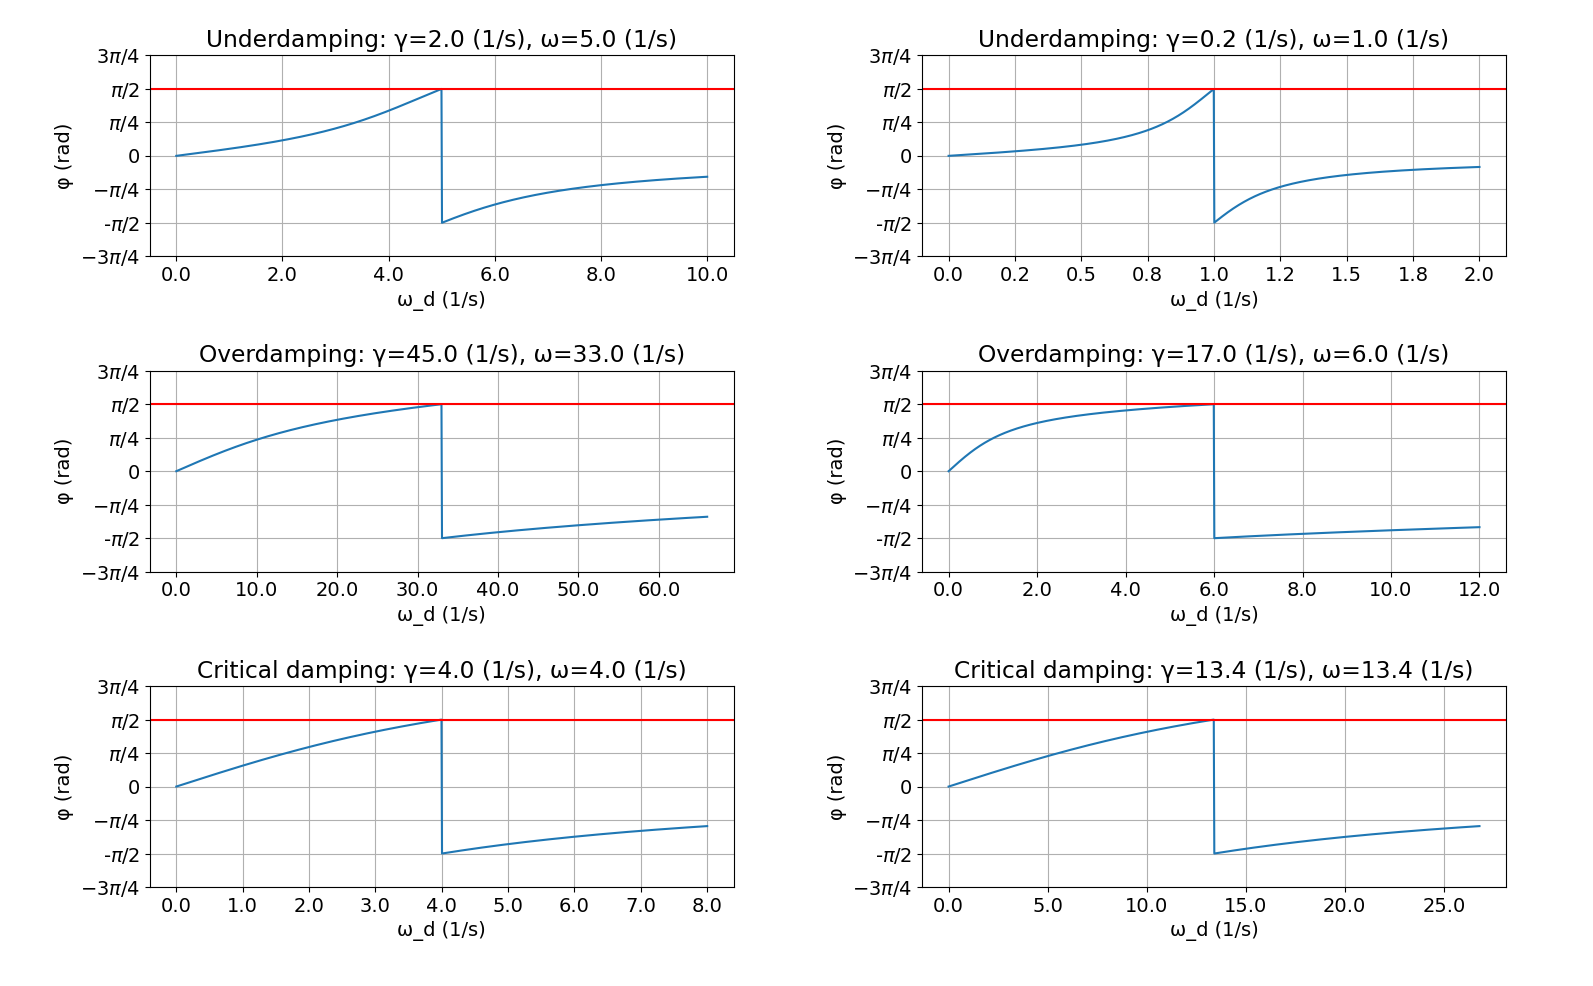
\includegraphics[width=1\textwidth]{oscillations/images/prep_exercise_Q3}
  \caption{Plots of the phase $\phi$ for different values of the damping factor $\gamma$ and natural frequency $\omega$.} 
  \label{fig:prep:phase}
\end{figure}

In Fig.~\ref{fig:prep:phase}, this discontinuity is clear for different initial conditions ($\gamma$ and $\omega$). If the driving frequency $\omega_d$ approaches natural frequency $\omega$ from the negative side, the phase $\phi$ approaches $\pi/2$ radians. In other words, the driving force becomes more out of phase with the natural oscillations. Identical reasoning applies to the positive half limit.
